\documentclass[a4paper,12pt]{article}
\usepackage{amsmath}
\usepackage[utf8]{inputenc}  
\usepackage{graphicx}       
\usepackage{geometry}
\usepackage{parskip}
\usepackage{textcomp}
%\usepackage{fontspec}
\usepackage{wrapfig}
\usepackage{caption}
\usepackage{listings}
\usepackage{xcolor}

\definecolor{darkgreen}{rgb}{0.0, 0.5, 0.0}
\lstdefinelanguage{RAPID}{
  morekeywords={MODULE, PROC, VAR, CONST, IF, THEN, ELSE, WHILE, FOR, TO, ENDFOR, RETURN, TRUE, FALSE, PERS, TASK, ENDPROC, ENDIF, ENDWHILE, TEST, CASE, DEFAULT, ENDTEST, STOP, ERROR, TRAP, CONNECT, DISCONNECT, RAISE, EXIT, ENDTRAP, WITH},
  sensitive=true,
  morecomment=[l]{!},       % Single-line comment
  morecomment=[s]{/*}{*/},   % Multi-line comment
  morestring=[b]{"}         % Strings wrapped in "
}

\lstdefinestyle{rapidstyle}{
  language=RAPID,
  basicstyle=\ttfamily\footnotesize,
  keywordstyle=\color{blue}\bfseries,
  stringstyle=\color{red},
  commentstyle=\color{darkgreen},
  numbers=left,
  numberstyle=\tiny,
  frame=single,
  backgroundcolor=\color{gray!10},
}

\lstset{style=rapidstyle}

\geometry{a4paper, margin=2.5cm} 

\begin{document}

\begin{titlepage}
    \centering
    \pagenumbering{gobble}
    \vfill
    
    \title{ABB RobotStudio, YuMi Application \& YuMi Challenge \\ \large TEL200 technical report}
    \author{J\o rgen Asmundvaag \\ Ludvik H\o iberg-Aslaksen \\ Christopher Ljosland Strand}
    \date{March 2025}
    \maketitle
    
    \vfill
\end{titlepage}

\pagenumbering{arabic}

\newpage
\tableofcontents

\newpage
\section{Abstract}
This lab project consists of two problems meant to solve with the ABB YuMi IRB® 1400 collaborative robot. 

YuMi Application i
The purpose of the YuMi Application is to move geometric objects to another position, and back to their position. This is achieved by applying the 

\section{Introduction}
Industrial robotics plays an increasingly vital role in enhancing productivity, precision, and efficiency within modern manufacturing processes. ABB RobotStudio and RAPID provides a powerful platform for simulating and optimizing robotic operations in a virtual environment prior to physical implementation.

In this project, we use ABB's RobotStudio simulation environment to develop, simulate, and deploy two different applications as described in the task description. 

The first application involves precisely picking up objects and moving them to another designated location at the click of a button, with additional safety functionality integrated through an emergency button.

The second application is the YuMi challenge where we were given an open task to test the capabilities of the YuMi robot. Inspired by the 18th century famous machine that fascinated audiences across Europe, "The Turk". As The Turk, we won´t either play fully autonomous and will use scholar´s mate to make it possible to finish within the given time frame. This  will provide an understanding of the functionality of YuMi robot and it´s capabilities doing precise tasks.

The report provides detailed insights into the methods, procedures, and results achieved through these applications, emphasizing practical experiences and theoretical connections drawn from the course syllabus.

\section{Method}
\subsection{Theory}
In this chapter, some important concepts are presented to help understand how a robotic arm moves.

\subsubsection{Pose in 3 dimensions}
The pose of an object describes its position and orientation relative to a known reference point. It can be mathematically represented using a homogeneous transformation matrix:

\[
T = 
\begin{bmatrix}
R & t \\
0 & 1
\end{bmatrix}
\]

- \( R \) represents orientation (rotation matrix).
\\
- \( t \) represents position (translation vector).

In two-dimensional (2D) space, the homogeneous transformation matrix is:
\[
T =
\begin{bmatrix}
r_{11} & r_{12} & x \\
r_{21} & r_{22} & y \\
0 & 0 & 1
\end{bmatrix}
\]

In three-dimensional (3D) space, the matrix expands to:
\[
T = 
\begin{bmatrix}
r_{11} & r_{12} & r_{13} & x \\
r_{21} & r_{22} & r_{23} & y \\
r_{31} & r_{32} & r_{33} & z \\
0 & 0 & 0 & 1
\end{bmatrix}
\]

\subsubsection{Path and Trajectory}
A path describes how the robot moves from one pose to another without specifying timing details. A trajectory, however, is a path combined with timing information, specifying when and how quickly the robot moves through each point along the path.

\subsubsection{Joint space vs. Cartesian space}
When moving the robotic arm, you must decide whether to calculate the motion using joint space or Cartesian space:

- \textbf{Joint space} describes the robot's position based on its joint angles. Paths in joint space are mathematically simple to compute but usually don't result in straight-line paths for the robot's tool. This can cause problems for tasks that require precise linear movements, like welding. Because joint space plans motion based solely on joint angles, the end-effector's actual path can differ from what is desired.

- \textbf{Cartesian space} directly considers the position of the robot's tool (end-effector). Cartesian paths ensure more precise, straight-line movements, ideal for tasks needing high accuracy. However, these calculations are more complex and may lead to very high joint velocities, particularly near singularities, which are positions where the robot has limited movement capabilities and might struggle to perform smooth motions.

\subsubsection{Singularities}
Singularities are specific robot poses where it loses the ability to freely move in certain directions. Near singularities, joint velocities can become very high, potentially causing mechanical issues or imprecise movements.

The YuMi robot, with its seven joints, experiences fewer singularities and can easily reach most points within its workspace, making it highly suitable for versatile tasks. Robots specifically designed for a certain task may not require many joints, but their reduced flexibility might cause problems if their operating conditions change unexpectedly.



\subsection{YuMi Application}
The workstation is composed of a cube, cylinder and prism and two slots for each where the task it to move these from one of the slots to the other one and back on the press of a button.
The YuMi application will not need any modifications to the models as these were already implemented.
\subsubsection{Creating the paths and targets}
the slots are places in a 3x3 grid where the coloums (x axis) is the slots and the rows (y axis) are the slots for each body, coordinate system defined from the table. The distance between the center of each slot is 100 mm. The task is to move the bodies from col 1$\rightarrow$3 or vice-versa. 
As the gripper has a local coordinate system and as the gripper will try to match its coordinate system with body we have to rotate all the points local coordinate system 180 degrees, either x or y (we used x).
Grabbing the cube is quite simple, we defined one point lower where it´s grabbing the cube and one above, each side, to avoid collision with the slots and/or drag. The path used these points to move the body from one side to the other.
Cylinder is very similar and no need for much extra, but important to be centered for it to hold.
Prism differs slightly from the other objects, for grabbing the the prism you need to rotate the local coordinate system 90 degrees for it to grab on the corner and the middle on the side for it to hold.  

\subsubsection{Code Structure and Timings}
The upper section within the module contains all the defined targets and two important variables: speed and precision. These variables control the simulation's speed and the precision of the YuMi robot's movements.

The main part of the RAPID code consists of a continuously running while loop, ensuring constant execution. Inside this loop, multiple if statements check the status of buttons connected to the YuMi robot. Nested within these conditions are additional checks that determine the direction of movement for each object. Each of these statements calls specific functions to perform the required movements.

For example, when the green button \textit{di\_cube} is pressed, the program first determines the direction the cube should move, subsequently calling either the \textit{cube\_left\_right} or \textit{cube\_right\_left} functions. These functions guide the robot to an upper target point, open the gripper, move down to grasp the object, close the gripper, move back up, transfer to the opposite side, descend again, release the object, and finally return to the starting position.

The same logic and procedure apply similarly for the cylinder and prism.

\subsubsection{Creating The Mechanism Of The Emergency Button}
\begin{wrapfigure}{r}{0.25\textwidth}
  \label{fig:create_joint}
  \centering
  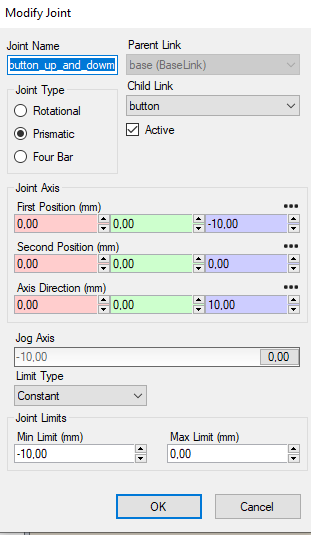
\includegraphics[width=0.2\textwidth]{create_joint.png}
  \caption{Create joint}
\end{wrapfigure}
The first step towards animating the button is to create a mechanism. This can be done by pressing the create mechanism button under the modeling tab, but first the emergency button needs to be two separate objects. To achieve this, right click then select disconnect library and then ungroup. After this has been done, the components will show up in create mechanism as components when creating joints. Under device dropdown select device and under the kinematic dropdown select other.

The second step is to create links and joints. First create the links with the e-stob base as the baselink, and the e-stop button as childlink. Then to create joints choose prismatic as the joint type and according to the task description the button has a travel distance of 10 mm. The button travels along the z-axis in the negative direction therefore the min limit is set to -10 mm and max limit to 0 mm. It is important to also set the first position to -10 mm. After this has been done the mechanism is done and compile mechanism can be pressed. The final step is to make a pressed pose such that it can be moved with smart components.

\subsubsection{Simulating The Emergency Button}
The emergency stop button needs to stop all movements when pressed and when let go, start all movement. To achieve this a trap routine must be used it has the ability to interrupt any movement then issue a command. The trap routine can be created using the syntax below:
\begin{lstlisting}
    TRAP EmergencyStop
        StopMove;
        WaitUntil di_EmergencySituation = 0;
        StartMove;
    ENDTRAP
\end{lstlisting}
This trap routine when called stops all movement then waits until the emergency button no longer is pressed. Under module a interrupt number needs to be defined this allows the program to use a interrupt in the code. This can be done by writing: 
\begin{lstlisting}
VAR intnum stop_emer; ! interrupt number datatype
\end{lstlisting}
After this the interrupt number stop\_emer needs to be connected to a trap routine. Using the CONNECT keyword can achieve this it also needs to be defined as the correct interrupt signal type this can be doing by using ISignalDI. All of this needs to be written under main.
\begin{lstlisting}
    ! Connects the intnum with the trap routine EmergencyStop
    CONNECT stop_emer WITH EmergencyStop;
    ! Handles checking wether the emergency stop button is pressed
    ISignalDI di_EmergencySituation, high, stop_emer;
\end{lstlisting}

When simulating the emergency button a digital output signal is required so that the di\_EmergencySituation can be set high while the button moves in the simulation. Create a digital output signal named do\_EmergencySituation with access level all. To simulate the movement of the button a input, a output a NOT logic gate and two pose movers are required in a smart component. 

When a pose mover receives a high signal to its Execute it will move the mechanism to that pose. Using a NOT gate the Execute on the pose mover can be set to high when the input is low such the unpressed state is active when input is low. The input is connected directly to pose mover for the pressed state so the pose mover will be in its pressed pose when the input is high. The input is also connect to directly to the output for use later in station logic. See figure~\ref{fig:smart_component_emer} for a picture of the smart component.
\begin{center}
    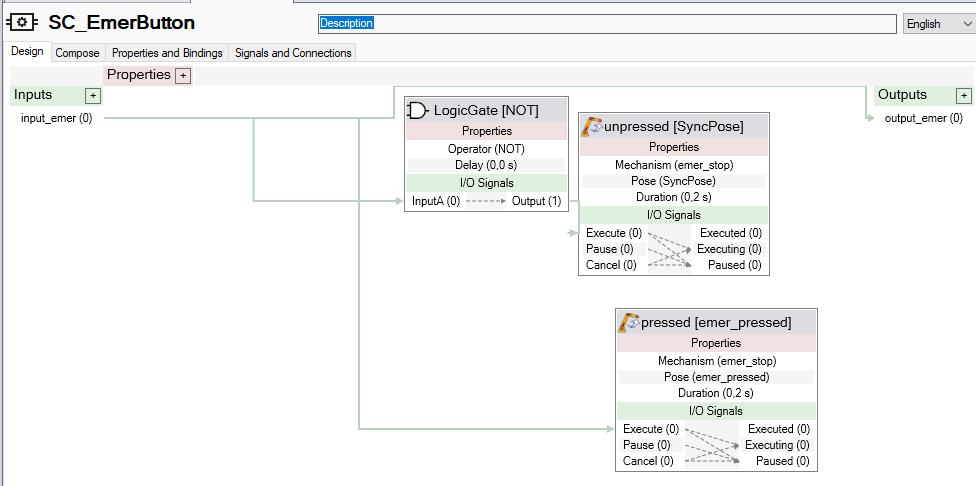
\includegraphics[width=0.8\linewidth]{SC_emer_button.png}
    \captionof{figure}{Smart component of the emergency button}
    \label{fig:smart_component_emer}
\end{center}
To connect the functionality of the emergency button to the simulated movement a few connections in station logic is required. First connect do\_EmergencySituation to input of the emergency button smart component then connect the output of the emergency button smart component to di\_EmergencySituation. When do\_EmergencySituation is set to high the button will move and execute the trap routine.

\subsection{YuMi Challenge}
\subsubsection{CAD geometry}
To be able to get accurate placements of the chess pieces, we modeled a chess board using the Rectangle surface geometry option in RobotStudio. Here we created a 25x25mm square surface, and created a chess board from 64 of these. We centered the board axis to align with the target of the wobj0, to simplify our setup process. We also aligned the border of the board 200 mm from the wobj0 target. 
We created targets for the center of each chess board square, to place the pieces correctly. 

To create our CAD geometry we used a 3D-scanner borrowed from Eiklab to make a 3D object of each type of chess piece. We then imported each 3D file into Fusion360 where we performed the following steps.
\begin{enumerate}
    \item Mesh $\rightarrow$ Insert $\rightarrow$ Insert Mesh
    \item Rotated the chess pieces such that they are straight
    \item Exported them as .sat files
\end{enumerate}
We then imported the .sat files into Robotstudio using the import CAD geometry button. When the chess pieces are imported we needed to move them their correct spaces on the chess board. This was done by trial and error, and duplicate button was used to get pieces which have multiples.

\subsubsection{Creating the paths and targets}
\label{sec:Challenge_paths_targets}
When creating the paths, we based the targets on the following chess moves.

\begin{table}[h] %Scholar's mate moves
    \centering
    \begin{tabular}{c l l}
        \hline
        Move & White & Black \\
        \hline
        1. & e4 & e5 \\
        2. & Dh5 & Sc6 \\
        3. & Lc4 & Sf6?? \\
        4. & Dxf7 & (checkmate) \\
        \hline
    \end{tabular}
    \caption{Scholar's Mate}
    \label{tab:chess_moves}
\end{table}
To make the YuMi Robot's moves as clean as possible it is important to have two targets above the desired destination. One that is about 5 mm above the chess piece and one that is higher in the range 25-50 mm above the piece. This allows the YuMi Robot to move smoothly between each target. Due to the 3D-scans being somewhat inaccurate the distances specified before may need some adustments depending on the piece and quality of the model.

To simplify the paths the YuMi Robot returns to a set point after picking up or placing a piece. This point is centered above the queen with a 25 mm offset towards the YuMi Robot. 

After the paths have been created it is important to note that a fully extended gripper would collide with pieces surrounding the piece to be picked up. To solve this the rapid command \textit{g\_MoveTo value;} was used. This command extends the gripper to the specified value allowing the gripper to easily slide between the pieces. The space between chess pieces is about 7 mm for the large pieces and about 8 mm for pawns.

After YuMi robot has won the game it will do a little victory dance by simply moving the arm up in the air up and down. To get this to work it also has to be implemented a helping point, as moving from start position straight up would cause a collision. Therefore, by putting a helping point in front and up from the robot then returning back to y axis it will be able to safely perform the victory dance. 

\subsubsection{Code structure and timings}
The top part located within the module part consist of all the targets and two variables called speed and precision. The variables control the simulation speed and precision of the YuMi Robot. The main body of the Rapid code consists of while loop that is constantly true allowing the code to run in a loop, within the while loop the code has several if statements that check if the buttons connected to the YuMi Robot are pressed. These if statements contain the different functions for each chess move.

The green button \textit{di\_cube} when pressed runs move 1 chess move from table~\ref{tab:chess_moves}. When it is pressed a second time it runs move 2 and so on. After all moves are run it resets to move 1. The second blue button \textit{di\_cylinder} runs all moves with timing delay specified in the code by a variable. The third red button \textit{di\_prism} runs the celebration described in section \ref{sec:Challenge_paths_targets}. The fourth yellow button \textit{di\_home} returns the YuMi Robot to its start position.

The final button is an emergency stop button called \textit{di\_EmergencySituation} this button when pressed runs a trap routine that stops the YuMi Robot mid path, and when let go it starts to move from the same position it stopped. One of the main perks to using a trap routine is that it can interrupt any movement and then issue a command which the it would not be able to do with if statements.

\subsubsection{Physical development}
To get a chess board with the same size and targets as the one used for the simulation, we had to create it from scratch. For this we used Figma, and created an A4 frame, with 25x25mm squares. To get the correct placement of the pieces, we created a cross in the center of each square. This got exported as a pdf, and printed out. 

\section{Results}
\subsection{YuMi Application}
For the YuMi Application task, we found several results during our work on the robot. By applying the knowledge on poses and joints from the lectures, we managed to move all the geometric forms both to the other side, and back to their starting position. 

\subsubsection{Challenges}
The greatest challenge we faced during our work on the YuMi Application, was in regards to poses and singularities. 
The YuMi has 7 degrees of freedom and is a redundant manipulator. This gives the 

\subsection{YuMi Challenge}
For the YuMi Challenge, we managed to play the Scholar's mate against a person, using the collaborative 
\subsubsection{Challenges}

After achieving a working simulation, we tested it on the actual robot, but encountered issues not present in the simulation. Movements that functioned well in simulation caused collisions or exceeded joint limits in practice. To address this, intermediate help points can be added to guide the robot safely around obstacles. However, the primary issue usually arises from inconsistent axis configurations across target points, causing unexpected rotations or joint over extensions. Ensuring consistent axis configurations for all points within the same path effectively resolves this problem.

\subsection{YuMi Challenge}
The YuMi challenge did not present significant issues regarding configurations; however, we encountered challenges related to the precision required when playing chess with a robotic arm. Specifically, ensuring that the arm or gripper avoided accidental contact with other pieces while grabbing or placing chess pieces demanded careful attention. To resolve this, we adjusted the height of the arm movements to prevent unwanted contact. During placement, problems arose from either missing the intended target or unintentionally knocking over adjacent pieces, largely because such conditions weren't visible in simulations. Introducing helping points or raising the pieces slightly mitigated these difficulties.
Additionally, we encountered an issue where the gripper had sticky tape on it, causing pieces to become stuck during handling. 
After these issues were tackled it worked flawlessly and the victory dance added at the end also worked as intended.

\section{Discussion}
\subsection{YuMi Application}
\subsubsection{Paths}
One area we could have improved, would be on the paths that the robot are following. We have seen improvements in every version of our program, and we feel that the paths that ended up being in the program are the simplest and most linear we have managed to create. But there are definetily an area of improvement, especially for clearance. Even though the robot is moving clear of any objects and collisions, we are aware of some positions on the path where the arm could benefit from more distance from both the table and the robot body.

\subsection{YuMi Challenge}
\subsubsection{Expansion}
For the YuMi Challenge, we decided to hard code the moves of the common schools´ mate. Although we think this is sufficient to show of the YuMi´s application in a collaborative environment in regard to the time at hand, we see the possibility to expand its moves and gameplaying ability. 

Before deciding on defining the moves as paths, we explored the possibility of using the buttons as forward/backward, left/right and pick up/down buttons. This would emulate a game controller, making it possible to play all possible moves.  


\section{Conclusions} 
The ABB YuMi 1400 cobot is powerful and versatile. During the projects we have seen both its capabilities and its limitations. 
having the opportunity  to develop in RobotStudio, test our code on the robot, debug and go back to RobotStudio abled us to quickly patch bugs, test new approaches and refine our code. 

For the YuMi Challenge, having the freedom to choose our task, gave us another view on working with cobots, and
\end{document}
